\documentclass[a4paper]{article}

% Set up page size
\usepackage[margin=1.5cm, includefoot, footskip=30pt]{geometry} 

% Nice way to display code
\usepackage{minted}

% Import images
\usepackage{graphicx}
\usepackage{amsmath}
\usepackage{multicol}

\title{The Monty Hall problem and the effect of goats}
\author{Vince Knight}
\date{}


\begin{document}
\maketitle

\section{Introduction: The Monty Hall Problem}

The Monty hall problem is a probabilistic problem based on a game
show~\cite{rosenhouse2009monty}. In this show a contestant was presented with
three doors. Behind one of the doors was a car and behind the others was a
goat. The contestant would choose a door (which would thus either be hiding a
goat or a car) and the host would then open a door showing the location of the
goat. At this stage the contestant had a strategic choice:

\begin{itemize}
    \item Stick: if their original choice had the car they won!
    \item Switch: take whatever was behind the remaining door.
\end{itemize}

This puzzled many mathematicians for years as it might seem that the contestant
is given a false choice and the probability of winning is in fact the same
whether or not they switch. This is however not true: if the contestant
switched they doubled their probability of winning!

In this work, we will hopefully clarify this by considering what happens if we
modify the game: let us have \(n\) goats behind \(n\) doors. Everything else
remains the same: the host still opens one of the doors behind which is a goat.

In Section~\ref{sec:simulation} Python will be used to simulate both strategies
and find the probability of winning. Then in
Section~\ref{sec:analytical_formulae} a mathematical formula for the probability
of winning will be obtained and verified.

\section{Simulating more goats}\label{sec:simulation}

Here are two python functions that simulate sticking or switching with a given
number of goats:

\begin{minted}{python}
import random

def stick(number_goats=2):
    """A function to simulate a play of the game when we stick"""
    doors = ['Car'] + number_goats * ['Goat']
        
    initial_choice = random.choice(doors)  # make a choice
    return initial_choice == 'Car'

def switch(number_goats=2):
    """A function to simulate a play of the game when we swap"""
    doors = ['Car'] + number_goats * ['Goat']  
    
    initial_choice = random.choice(doors)  # make a choice
    
    doors.remove(initial_choice)  # Switching: remove initial choice
    doors.remove('Goat')  # The game show host shows us a goat
    
    new_choice = random.choice(doors)   # We choose our one remaining option
            
    return new_choice == 'Car'
\end{minted}

Using this we can simulate the probabilities for the case of 2 goats (the
original TV show!):

\begin{minted}{python}
>>> repetitions = 10000
>>> random.seed(0)
>>> prob_win_stick = sum([stick() for rep in range(repetitions)]) / repetitions
>>> prob_win_switch = sum([switch() for rep in range(repetitions)]) / repetitions
>>> prob_win_stick, prob_win_switch
(0.3346, 0.6636)
\end{minted}

This indeed looks like the contestant is twice as likely to win if they switch.

\section{Analytic formulae}\label{sec:analytical_formulae}

We can compute the probability \(p_n\) of winning when switching when there are
\(n\) goats. In order to win when switching:

\begin{itemize}
    \item The initial choice must not be the car. If there are \(n\) goats,
        there are a total of \(n + 1\) doors. Thus, the probability of finding
        the car is \(\frac{1}{n + 1}\). Thus, the probability of \textbf{not}
        finding the car is \(1 - \frac{1}{n + 1}\).
    \item Switching implies choosing the car from the remaining doors. There
        have however been 2 doors removed (the original choice and the one that
        the host opens). Thus the probability of choosing the car is
        \(\frac{1}{n - 1}\).
\end{itemize}

Thus:

\begin{multicols}{2}

    \begin{align}
        p_n &= \left(1 - \frac{1}{n + 1}\right)\left(\frac{1}{n - 1}\right)\\
        p_n &= \left(\frac{n + 1 - 1}{n + 1}\right)\left(\frac{1}{n - 1}\right)\\
        p_n &= \frac{n}{(n + 1)(n - 1)}\\
        p_n &= \frac{n}{(n^2 - 1)}
    \end{align}

    \columnbreak

Using Python to verify the algebra:

    \begin{minted}{python}
    >>> import sympy as sym
    >>> n = sym.symbols('n')
    >>> p_n = (1 - 1 / (n + 1)) * (1 / (n - 1))
    >>> p_n.simplify()
    n/(n**2 - 1)
    \end{minted}

\end{multicols}

The ratio of how much better it is to switch is thus given by:

\[
    \alpha_n = \frac{p_n}{1 / (n + 1)} = \frac{n}{n - 1}
\]


Finally, let us compare this formulae to simulated values.

\begin{minted}{python}
def ratio(repetitions=50000, number_goats=2):
    """Obtain the ratio of win probabilities"""
    prob_win_stick = sum([stick(number_goats=number_goats) 
                          for rep in range(repetitions)]) / repetitions
    prob_win_switch = sum([switch(number_goats=number_goats) 
                           for rep in range(repetitions)]) / repetitions
    return prob_win_switch / prob_win_stick
\end{minted}

\begin{minted}{python}
\end{minted}

Here is some Python code that plots this ratio (both simulated and using the
formulae) shown in
Figure~\ref{fig:simulated_v_expected_ratio_of_win_probability}.

\begin{minted}{python}
>>> random.seed(0)
>>> goats = range(2, 25 + 1)
>>> ratios = [ratio(number_goats=n) for n in goats]
>>> theoretic_ratio = [(n / (n - 1)) for n in goats]
>>> plt.figure()
>>> plt.scatter(goats, ratios, label="simulated")
>>> plt.plot(goats, theoretic_ratio, color="C1", label="theoretic")
>>> plt.xlabel("Number of goats")
>>> plt.ylabel("Ratio")
>>> plt.legend()
>>> plt.savefig("simulated_v_expected_ratio_of_win_probability.pdf");
\end{minted}

\begin{figure}[!htbp]
    \begin{center}
        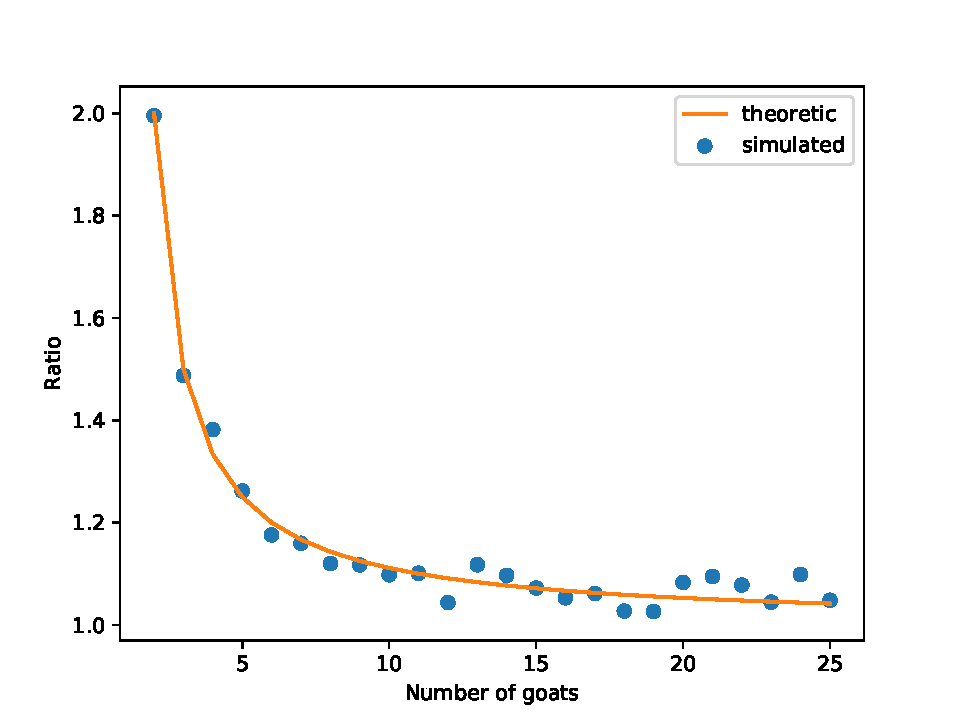
\includegraphics[width=.6\textwidth]{./simulated_v_expected_ratio_of_win_probability.pdf}
    \end{center}
    \caption{The simulated and expected effect of goats on the win probability}
    \label{fig:simulated_v_expected_ratio_of_win_probability}
\end{figure}

Finally let us confirm that as the number of goats grows the effect of switching
gets smaller and smaller:

\begin{multicols}{2}

    \begin{align}
        \lim_{n\to\infty}\alpha_n & = \lim_{n\to\infty}\frac{n}{n - 1}\\
        \lim_{n\to\infty}\alpha_n & = \lim_{n\to\infty}\frac{1}{1 - 1 / n}\\
        \lim_{n\to\infty}\alpha_n & = 1
    \end{align}

    \columnbreak

Using Python to verify this calculation:

    \begin{minted}{python}
    >>> import sympy as sym
    >>> alpha_n = p_n / (1 / (n + 1))
    >>> sym.limit(alpha_n, n, sym.oo)
    1
    \end{minted}

\end{multicols}

\section{Conclusion}

This report has used mathematics and Python to shed some light on the Monty hall
problem. The modified version of the problem considers the effect of having a
given number of goats in the game.

An analytical formula is obtained for the probability of winning if the player
switches.

As the number of goats increases the beneficial effect of switching is reduced:
this makes intuitive sense as the increase of goats implies that the host makes
very little change to the problem by showing a door with a goat.

Other avenues for investigation could include seeing the effect of adding more
cars and also what happens when the host opens more doors with goats.

\bibliographystyle{plain}
\bibliography{bibliography.bib}

\end{document}
